\section{Introdução}
\label{sec:introducao}

O problema tratado neste trabalho é um desafio de xadrez com regras diferentes das habituais.
Dado um tabuleiro quadrado de lado $N$, com um dígito de 0 a 9 em cada casa, e um cavalo em
uma casa marcada com C, o objetivo é levar o cavalo até uma casa de saída, marcada com S, no
menor número possível de movimentos.

Duas regras tornam o problema diferente do xadrez comum. A primeira é que o dígito das casas
aumenta o pulo do cavalo: o dígito 0 corresponde ao pulo normal de xadrez, em forma de L, e
dígitos maiores esticam o L, como mostra a Figura~\ref{fig:pulos}. A segunda é que as bordas
do tabuleiro se encostam: se o cavalo sai pela direita, entra pela esquerda, e se sai por
cima, entra por baixo. Por isso diz-se que o tabuleiro é \emph{toroidal}.

\begin{figure}[ht]
  \centering
  % Figura 1: forma do pulo em L para os dígitos 0, 1 e 2.
%
% Como ler o código: cada L tem (2+d) passos na horizontal e (1+d) na vertical.
% As casas brancas formam o L do dígito 0; as casas coloridas são as d casas
% acrescentadas em cada perna. Para mudar as cores, edite \colorlet abaixo; para mostrar
% mais dígitos, acrescente um par "d/posição" na lista do \foreach (por exemplo 3/17.2).
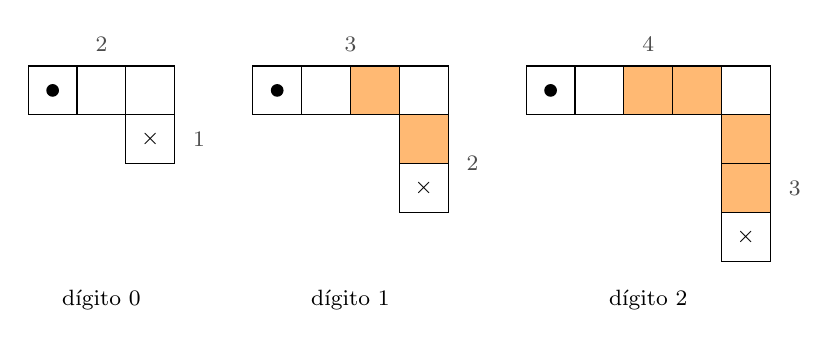
\begin{tikzpicture}[x=0.62cm,y=0.62cm,font=\footnotesize]
  \colorlet{extra}{orange!55}
  \foreach \d/\xo in {0/0, 1/4.6, 2/10.2} {
    \pgfmathtruncatemacro{\pl}{2+\d}   % passos na horizontal = coluna do canto
    \pgfmathtruncatemacro{\pc}{1+\d}   % passos na vertical
    % perna horizontal (linha de cima)
    \foreach \c in {0,...,\pl} {
      \pgfmathtruncatemacro{\ex}{and(\c>=2,\c<\pl)}
      \ifnum\ex=1 \def\cor{extra}\else\def\cor{white}\fi
      \draw[fill=\cor] ({\xo+\c},0) rectangle ++(1,1);
    }
    % perna vertical (abaixo do canto)
    \foreach \r in {1,...,\pc} {
      \pgfmathtruncatemacro{\ex}{\r<=\d}
      \ifnum\ex=1 \def\cor{extra}\else\def\cor{white}\fi
      \draw[fill=\cor] ({\xo+\pl},{-\r}) rectangle ++(1,1);
    }
    % casa de partida (ponto) e casa de chegada (x)
    \fill ({\xo+0.5},0.5) circle (0.13);
    \node at ({\xo+\pl+0.5},{-\pc+0.5}) {$\times$};
    % comprimento de cada perna, em passos
    \node[gray!60!black] at ({\xo+(\pl+1)/2},1.45) {\pl};
    \node[gray!60!black] at ({\xo+\pl+1.5},{-\pc/2}) {\pc};
    % rótulo do dígito
    \node[anchor=north] at ({\xo+(\pl+1)/2},-3.4) {dígito $\d$};
  }
\end{tikzpicture}

  \caption{Forma do pulo para os dígitos 0, 1 e 2. As casas brancas formam o L do dígito 0, e as
  casas coloridas são as $d$ casas acrescentadas em cada perna. O ponto é a casa de partida, o
  $\times$ é a casa de chegada, e os números indicam o comprimento de cada perna, em passos.}
  \label{fig:pulos}
\end{figure}

O enunciado traz um tabuleiro de exemplo, com 10 linhas e 10 colunas
(Figura~\ref{fig:exemplo}), e informa que nele o cavalo vai de C a S em 3 pulos. Esse
exemplo é usado ao longo do relatório para explicar e conferir o algoritmo.

\begin{figure}[ht]
  \centering
  \ttfamily
  \begin{tabular}{@{}r@{\hspace{1.2em}}l@{}}
     & 0123456789\\
    0 & 4286305993\\
    1 & 67126514C1\\
    2 & 3541559238\\
    3 & 6344361236\\
    4 & 0419867802\\
    5 & 4271613350\\
    6 & S668962685\\
    7 & 6244051139\\
    8 & 3714702030\\
    9 & 0084825587\\
  \end{tabular}
  \caption{Tabuleiro de exemplo do enunciado. Linhas e colunas são numeradas de 0 a 9, a partir do
  canto superior esquerdo: C está na linha 1, coluna 8, e S na linha 6, coluna 0.}
  \label{fig:exemplo}
\end{figure}

Cada caso de teste é um arquivo de texto com $N$ linhas de $N$ caracteres: dígitos de 0 a 9,
exatamente um C e exatamente um S (isso foi conferido nos oito arquivos). Para cada caso, a saída
é o menor número de movimentos de C até S, ou a palavra ``impossível'' quando S não pode ser
alcançada. Os oito tabuleiros vão de $40 \times 40$ a $1500 \times 1500$ casas, e o maior
deles tem mais de dois milhões de casas.

O enunciado não exige recursão, e a solução apresentada usa um laço com uma fila, pelos
motivos explicados na Seção~\ref{sec:algoritmo}.

Este relatório está organizado da seguinte forma: a Seção~\ref{sec:modelagem} mostra como o
problema foi modelado, incluindo a regra do pulo e o tratamento do toro; a
Seção~\ref{sec:algoritmo} apresenta o algoritmo, com um exemplo passo a passo; a
Seção~\ref{sec:eficiencia} analisa a eficiência; a Seção~\ref{sec:resultados} mostra os
resultados dos oito casos e como eles foram conferidos; e a Seção~\ref{sec:conclusao} traz as
conclusões.
